\begin{center}
    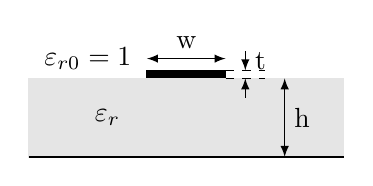
\begin{tikzpicture}
        %Leiterbahn
        \filldraw[black]    (1,1)   rectangle (2,1.1);
        %Dielektrika
        \filldraw[black!10] (-.5,0) rectangle (3.5,1);
        \draw[-,thick](-.5,0)--(3.5,0);
        %Bemassungen
        \draw[latex-latex](2.75,0)--(2.75,1) node[midway, right]{h};
        \draw[latex-latex](1,1.25)--(2,1.25) node[midway, above]{w};
        \draw[dashed](2,1)      --(2.5,1);
        \draw[dashed](2,1.1)    --(2.5,1.1);
        \draw[latex-](2.25,1)   --(2.25,.75);
        \draw[latex-](2.25,1.1) --(2.25,1.35) node[midway, right]{t};
        %Dielektrizitätskonstanten
        \node at (.5,.5)[]{$\varepsilon_r$};
        \node at (.25,1.25)[]{$\varepsilon_{r0}=1$};
    \end{tikzpicture}
\end{center}
